\section{$C^1$ Finite Element Discretisation}
\label{sec:fem}

\subsection{Bogner--Fox--Schmit Bicubic Hermite Element}
In Mindlin Form-II gradient elasticity, the weak form of equilibrium requires square-integrable second derivatives of displacement, placing the variational space in the Sobolev space $H^2(\Omega)$. Consequently, standard $C^0$-continuous Lagrange elements are non-conforming and suffer from severe convergence pathologies. To guarantee conforming $C^1$ inter-element continuity across rectangular element boundaries, we adopt the Bogner--Fox--Schmit (BFS) bicubic element \cite{bfs1965}.

For a rectangular element of dimensions $2a \times 2b$, the displacement components $u_1(x, y)$ and $u_2(x, y)$ are interpolated independently as tensor products of one-dimensional cubic Hermite polynomials:
\begin{equation}
u_i(x, y) = \sum_{a=1}^4 \sum_{p=1}^4 N_{a,p}(x, y) d_{i, a, p}^e, \quad i \in \{1, 2\},
\label{eq:bfs_interpolation}
\end{equation}
where $a \in \{1, 2, 3, 4\}$ indexes the four element vertices, and $p \in \{1, 2, 3, 4\}$ denotes the four nodal degrees of freedom per displacement component:
\begin{equation}
\bm{d}_{i, a}^e = \begin{bmatrix} u_i & \frac{\partial u_i}{\partial x} & \frac{\partial u_i}{\partial y} & \frac{\partial^2 u_i}{\partial x \partial y} \end{bmatrix}^\mathsf{T}_{\text{at node } a}.
\label{eq:nodal_dof_vector}
\end{equation}
With 4 vertices and 2 displacement components, each BFS element contains $4 \times 2 \times 4 = 32$ degrees of freedom. Figure~\ref{fig:bfs_dof} illustrates the nodal DOF arrangement and the complex phase mapping on periodic boundaries. All band-structure and design-map results reported below are computed with a uniform mesh of $n \times n = 16 \times 16$ BFS elements per unit cell ($h = L/n = 0.0625$, hence $8 n^2 = 2048$ degrees of freedom per cell); the element order $n$ is listed in Table~\ref{tab:case_params}.

\begin{figure}[htbp]
\centering
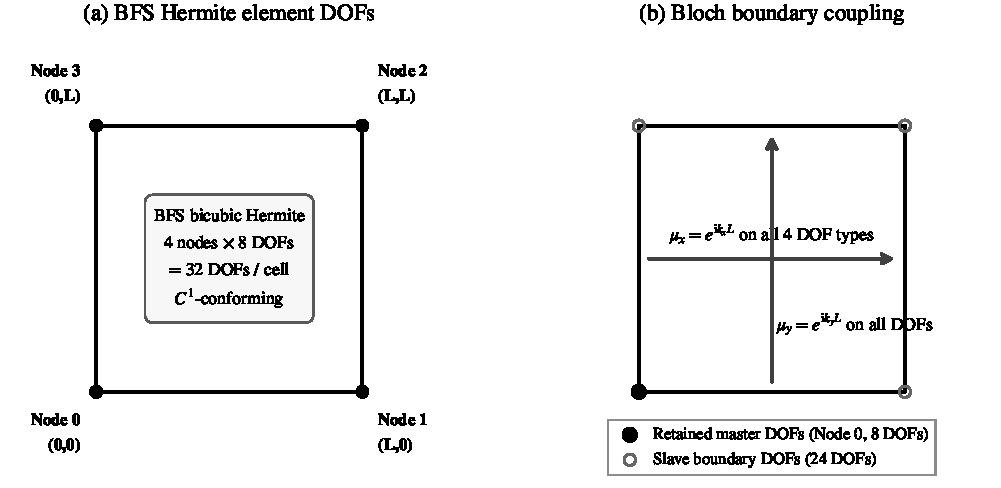
\includegraphics[width=\textwidth]{figures/fig03_bfs_dof_bloch.pdf}
\caption{(a) Degree-of-freedom structure of the 32-DOF $C^1$ Bogner--Fox--Schmit (BFS) bicubic element, showing 4 nodal DOFs $\{u, u_{,x}, u_{,y}, u_{,xy}\}$ per displacement component. (b) Master--slave Bloch periodic boundary coupling, illustrating identical phase transformation $e^{\iu \bmk \cdot \bm{a}_\alpha}$ applied across primary and derivative degrees of freedom.}
\label{fig:bfs_dof}
\end{figure}

\subsection{Element matrices}
The strain tensor $\bm\varepsilon$ and strain-gradient tensor $\bm\eta$ within element $e$ are related to the element nodal displacement vector $\bm{d}^e \in \mathbb{R}^{32}$ via kinematic strain-displacement matrices $\bmB^c$ and $\bmB^g_k$:
\begin{equation}
\bm\varepsilon = \bmB^c \bm{d}^e, \quad \bm\eta_k \equiv \frac{\partial \bm\varepsilon}{\partial x_k} = \bmB^g_k \bm{d}^e, \quad k \in \{1, 2\}.
\label{eq:strain_matrices}
\end{equation}
The total element stiffness matrix $\bmK^e$ separates cleanly into classical and gradient contributions:
\begin{equation}
\bmK^e = \bmK^c + \bmK^g(\theta, \mathrm{AR}),
\label{eq:Ke_total}
\end{equation}
where the classical stiffness matrix is:
\begin{equation}
\bmK^c = \int_{\Omega_e} (\bmB^c)^\mathsf{T} \bmC \bmB^c \,\dif\Omega,
\label{eq:Kc_int}
\end{equation}
and the anisotropic gradient stiffness matrix is:
\begin{equation}
\bmK^g(\theta, \mathrm{AR}) = \frac{1}{10} \sum_{k=1}^2 \sum_{l=1}^2 L_{kl}(\theta) \int_{\Omega_e} (\bmB^g_k)^\mathsf{T} \bmC \bmB^g_l \,\dif\Omega.
\label{eq:Kg_int}
\end{equation}
Because the shape functions are bicubic tensor-product polynomials, each homogeneous-element stiffness and mass integrand has degree at most six in each coordinate. A four-point Gauss--Legendre rule is exact through degree seven, so the $4 \times 4$ tensor rule is the smallest rule that integrates all such terms exactly. This avoids quadrature error for homogeneous elements; the unconstrained stiffness still has its expected rigid-body null modes. In elements cut by the inclusion, the discontinuous material field is instead integrated by sub-cell Gauss sampling with an $O(h)$ geometric approximation (Section~\ref{sec:caseC_pc}).

\paragraph{Mass and micro-inertia matrices.}
Similarly, the kinetic energy yields classical and micro-inertia mass contributions:
\begin{equation}
\bmM^e = \bmM_0 + \ell_{\mathrm{i}}^2 \bmM^g,
\label{eq:Me_total}
\end{equation}
with:
\begin{equation}
\bmM_0 = \rho \int_{\Omega_e} \bm{N}^\mathsf{T} \bm{N} \,\dif\Omega, \quad \bmM^g = \rho \sum_{k=1}^2 \int_{\Omega_e} \left(\frac{\partial \bm{N}}{\partial x_k}\right)^\mathsf{T} \left(\frac{\partial \bm{N}}{\partial x_k}\right) \,\dif\Omega.
\label{eq:Mg_int}
\end{equation}
Both $\bmM_0$ and $\bmM^g$ are symmetric and positive semi-definite; their sum $\bmM^e$ is strictly positive definite for any positive density $\rho > 0$.

\subsection{Bloch reduction and eigenproblem}
To apply the Bloch boundary conditions across the unit cell boundary $\partial\Omega_{\mathrm{cell}}$, the global degrees of freedom $\bm{d}$ are partitioned into interior ($I$), master boundaries ($M$), and slave boundaries ($S$):
\begin{equation}
\bm{d} = \begin{bmatrix} \bm{d}_I \\ \bm{d}_M \\ \bm{d}_S \end{bmatrix}.
\label{eq:d_partition}
\end{equation}
The slave degrees of freedom on the top and right boundaries are related to the corresponding master degrees of freedom on the bottom and left boundaries via the Bloch transformation:
\begin{equation}
\bm{d}_S = \bmT_{SM}(\bmk) \bm{d}_M,
\label{eq:slave_master_rel}
\end{equation}
where $\bmT_{SM}(\bmk)$ is a diagonal complex phase matrix formed by evaluating $e^{\iu k_x L}$, $e^{\iu k_y L}$, or $e^{\iu (k_x + k_y)L}$ for each periodic node pair. As derived in Section~\ref{sec:bloch}, identical phase factors apply to the displacement, first-order, and cross-derivative DOFs.

The continuous weak-form boundary work also cancels pairwise across opposite cell faces. The effective traction $p_i^{\mathrm{dyn}}$ defined in Section~\ref{sec:continuum} inherits the Bloch phase and reverses sign with the outward normal, while its test displacement carries the conjugate phase. The double traction $R_i=n_jn_k\tau_{ijk}$ inherits the Bloch phase but is unchanged by normal reversal; its work-conjugate normal derivative changes sign. Thus both face-work terms cancel. The associated line and corner terms pair under the same translations, including the product phase $e^{\iu(k_x+k_y)L}$ at the corner, so no independent free-boundary condition is imposed on a Bloch-paired face.

Defining the master-slave transformation matrix $\bmT(\bmk)$:
\begin{equation}
\bm{d} = \bmT(\bmk) \bar{\bm{d}}, \quad \bmT(\bmk) = \begin{bmatrix} \mathbf{I}_{II} & \mathbf{0} \\ \mathbf{0} & \mathbf{I}_{MM} \\ \mathbf{0} & \bmT_{SM}(\bmk) \end{bmatrix}, \quad \bar{\bm{d}} = \begin{bmatrix} \bm{d}_I \\ \bm{d}_M \end{bmatrix},
\label{eq:T_bloch}
\end{equation}
the reduced stiffness and mass matrices are obtained through Galerkin projection:
\begin{equation}
\bar{\bmK}(\bmk) = \bmT(\bmk)^\mathsf{H} \bmK \bmT(\bmk), \quad \bar{\bmM}(\bmk) = \bmT(\bmk)^\mathsf{H} \bmM \bmT(\bmk).
\label{eq:reduced_KM}
\end{equation}

\paragraph{Reduced Hermitian eigenproblem.}
The dispersion curves $\barw_n(\bmk)$ are determined by solving the reduced generalized eigenvalue problem:
\begin{equation}
\left[ \bar{\bmK}(\bmk) - \omega^2 \bar{\bmM}(\bmk) \right] \bar{\bm{d}} = \bm{0}.
\label{eq:eigenproblem}
\end{equation}
The diagonal phase subblock $\bmT_{SM}(\bmk)$ is unitary because each entry has unit modulus; the full map $\bmT(\bmk)$ is rectangular, has full column rank, and is not unitary. For positive elastic and inertial parameters, the full-cell matrices satisfy $\bmK\succeq 0$ and $\bmM\succ 0$. Their congruence projections therefore give Hermitian reduced operators:
\begin{equation}
\bar{\bmK}(\bmk)^\mathsf{H} = \bar{\bmK}(\bmk) \succeq 0, \quad \bar{\bmM}(\bmk)^\mathsf{H} = \bar{\bmM}(\bmk) \succ 0,
\label{eq:hermiticity}
\end{equation}
so the generalized eigenvalues $\omega_n^2$ are real and nonnegative. Furthermore, shifting $\bmk$ by a reciprocal lattice vector $\bm{G}$ leaves every Bloch phase unchanged and hence gives $\bar{\bmK}(\bmk + \bm{G}) = \bar{\bmK}(\bmk)$ and $\bar{\bmM}(\bmk + \bm{G}) = \bar{\bmM}(\bmk)$, ensuring exact periodicity across reciprocal space.

\paragraph{Branch tracking.}
Along high-symmetry path segments, band crossing occurs between modes of differing spatial symmetry. To maintain physical branch continuity and resolve mode identity, we employ the Modal Assurance Criterion (MAC) between modes at adjacent wave vectors $\bmk_1$ and $\bmk_2$. Let $\bm{d}_m(\bmk)=\bmT(\bmk)\bar{\bm{d}}_m(\bmk)$ be the corresponding full-cell eigenvector, and let $\bmM$ be the common, assembled full-cell mass matrix, including gradient micro-inertia. The cross-wavevector MAC is
\begin{equation}
\mathrm{MAC}_{mn}(\bmk_1,\bmk_2) = \frac{\left| \bm{d}_m(\bmk_1)^\mathsf{H} \bmM \bm{d}_n(\bmk_2) \right|^2}{\left( \bm{d}_m(\bmk_1)^\mathsf{H} \bmM \bm{d}_m(\bmk_1) \right) \left( \bm{d}_n(\bmk_2)^\mathsf{H} \bmM \bm{d}_n(\bmk_2) \right)}.
\label{eq:mac_def}
\end{equation}
Using lifted vectors gives both modes the same physical mass metric; the reduced mass matrix itself depends on $\bmk$ and is therefore not used as a common cross-wavevector metric. When the off-diagonal MAC indicates branch exchange, step-halving continuation is triggered. However, in accordance with standard phononic band-structure reporting, band gaps are formally evaluated using frequency-ordered eigenvalues $\barw_1(\bmk) \le \barw_2(\bmk) \le \dots \le \barw_N(\bmk)$, avoiding subjective mode-tracking ambiguities.
